Em uma folha de papel a reta $r$ passa pelo canto $A$ da folha e forma um ângulo $\alpha$ com a borda horizontal, como na figura 1.
Para dividir este ângulo $\alpha$ em três partes iguais, executaremos as
seguintes construções:

\begin{itemize}
\item[a)] inicialmente, marcamos dois pontos $B$ e $C$ sobre a borda vertical de modo que $AB$ = $BC$; pelo ponto $B$ traçamos a reta $s$ paralela à borda (figura 2);

\item[b)] a seguir, dobramos o papel, ajustando-o de modo que o ponto $C$ coincida com um ponto $C'$ sobre a reta $r$ e o ponto $A$ coincida com um ponto $A'$ sobre a reta $s$ (figura 3); chamamos de $B'$ o ponto com o qual $B$ coincide.

Mostre que as retas $AA'$ e $AB'$ dividem o ângulo $\alpha$ em três partes iguais.

\begin{center}
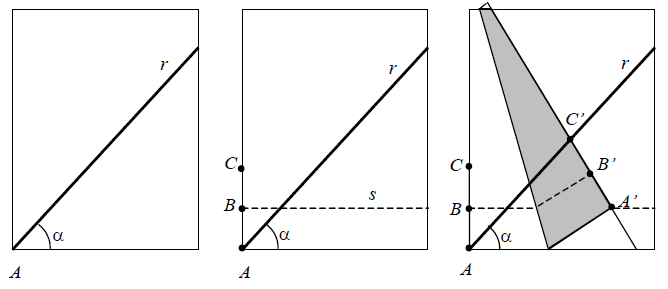
\includegraphics[width = 0.6\textwidth]{figura.png}
\end{center}

\end{itemize}